\documentclass[prl, article, twocolumn]{revtex4-1}

% packages
\usepackage[utf8]{inputenc}
\usepackage{graphicx}
\usepackage{amsmath}
\usepackage{amssymb}
\usepackage{subcaption}
\usepackage{minted}
\usepackage{fancyvrb}

% title
\begin{document}

\title{Classification, weight sharing, auxiliary losses}
\date{\today}
\author{Austin Zadoks}
\noaffiliation

\begin{abstract}
    Handwriting recognition and image comparison are posterchildren for the success of deep convolutional neural networks. In this report, I summarize a twin neural network implementation for predicting which digit is the greater in a pair of sub-sampled MNIST images. I also discuss the effects of weight sharing and auxiliary loss on the performance of the model. A twin neural network trained on 1000 image pairs over 25 epochs with weight sharing and auxiliary loss achieves an average test accuracy of 95.22~$\pm$~0.62~\% in FILL~$\pm$~FILL~seconds ($N=16$).
\end{abstract}

\maketitle

\section{Introduction}
The goal of this miniproject is to design a deep neural network which takes pairs of $14 \times 14$ grayscale images of handwritten digits from the MNIST database and predicts if the first digit is lesser or equal to the second digit.
Corresponding to each pair of images, we are given both a binary target which corresponds to whether the first digit is truly less than or equal to the second digit and the classes of the two digits in the image pair.

Given that we have knowlege of the classes of the two images, we can conceptually approach this problem in two steps: (1) construct a network which predicts the class of each of the images, and (2) construct a network which takes two outputs from the first network and predicts whether the digit in the first image is lesser or equal to that in the second.

To solve the first problem, a LeNet-5 style convolutional neural network is a good approach. For the second, a simple multilayer perceptron or fully-connected network should be both efficient and effective. If a convolutional network that uses the same weights is used for the first step, the overall network is called a twin network.

\section{Model architecture}
\begin{figure}[h!]
    \centering
    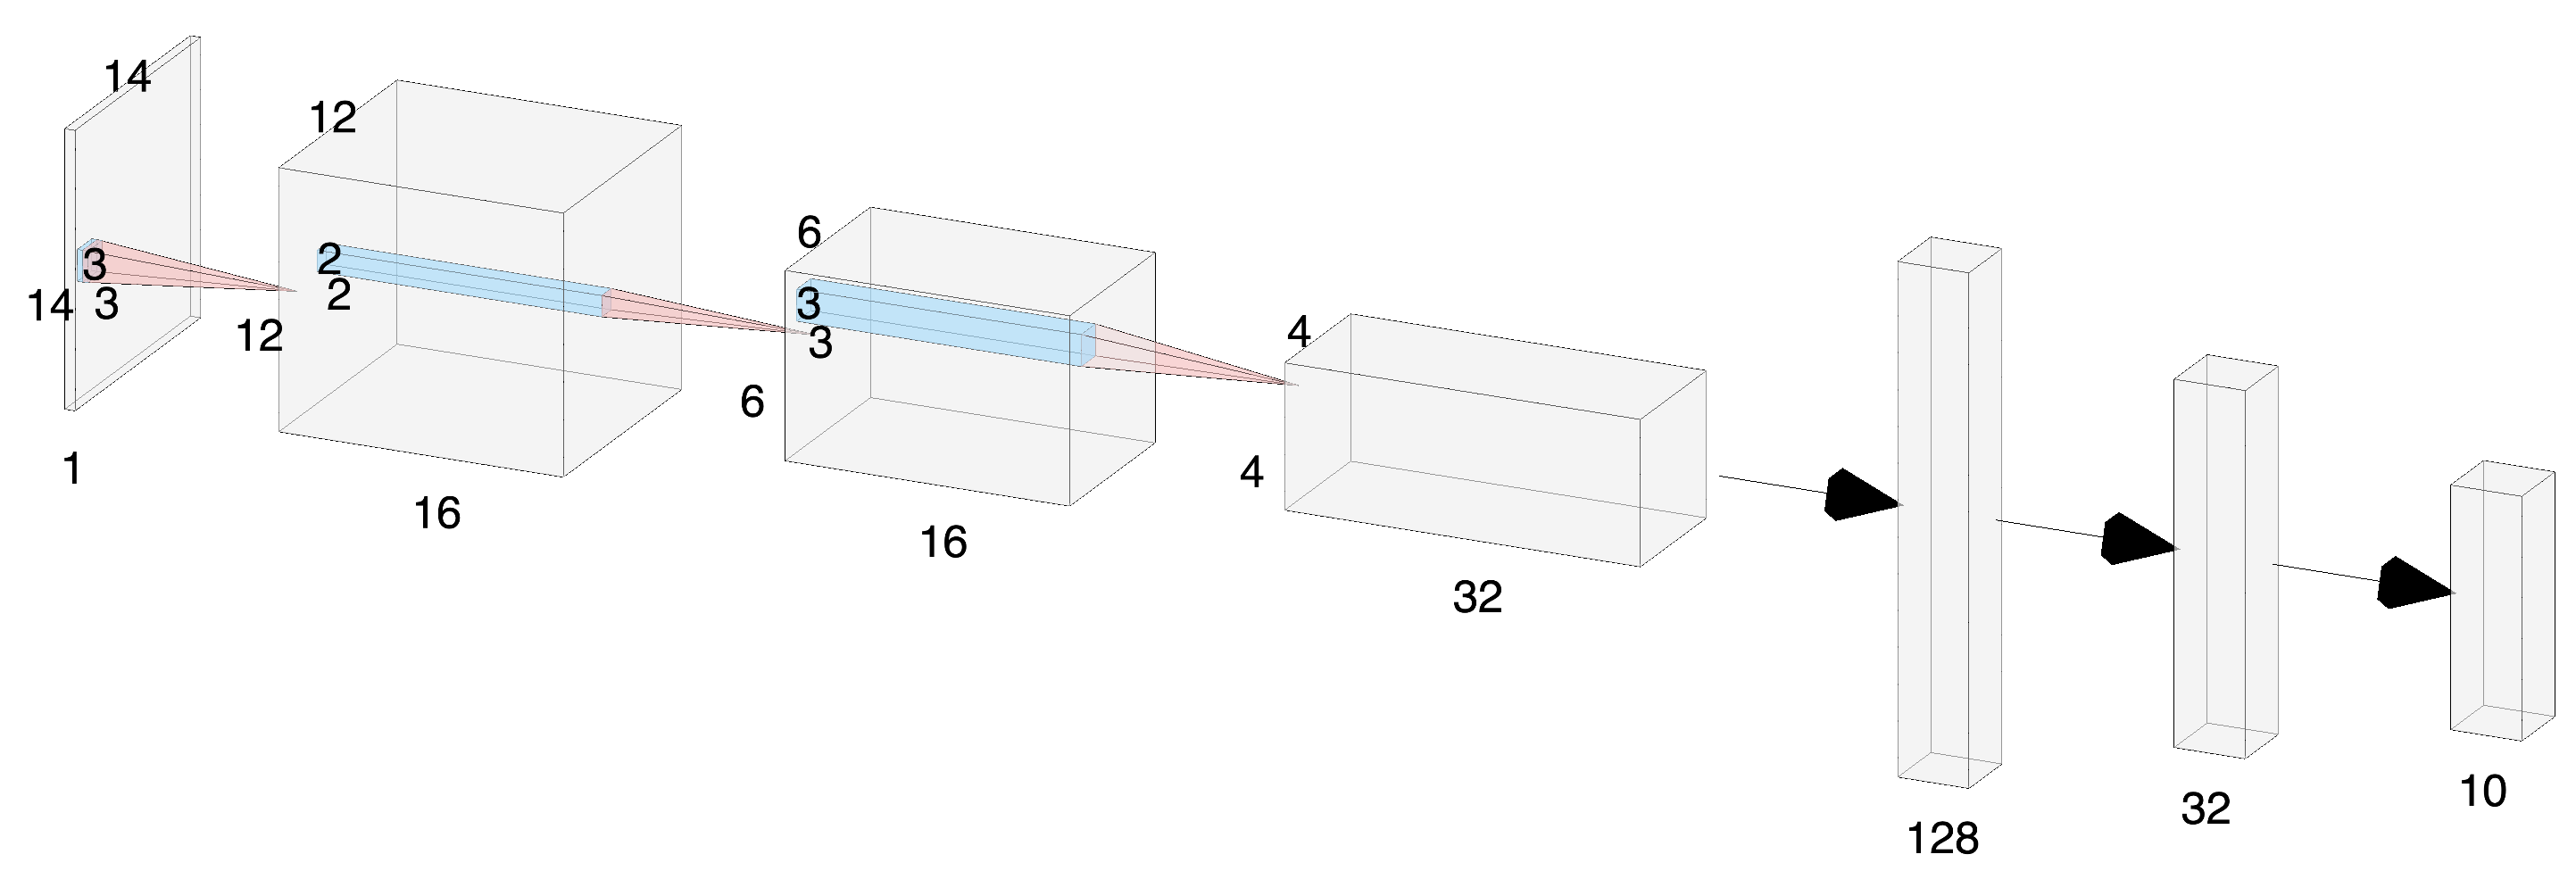
\includegraphics[width=\linewidth]{figures/LeNet.png}
    \caption{Convolutional subnet architecture}
    \label{fig:lenet}
\end{figure}

The convoluational subnet architecture, shown in Fig. \ref{fig:lenet}, takes in one image of shape $1 \times 14 \times 14$ and returns a vector of length $10$, containing the predicted categorization of the image as a digit 0-9. Written as an equivalent \texttt{torch.nn.Sequential} model, the convolutional subnet is:

\begin{minted}[fontsize=\small]{python}
import torch.nn as nn

nn.Sequential(
    nn.Conv2d(1, 16, 3),  # 3x3 to avoid aliasing
    nn.ReLU(),
    nn.AvgPool2d(2, 2),
    nn.Conv2d(16, 32, 3),  # "above"
    nn.ReLU(),
    nn.AvgPool2d(2, 2),
    nn.Flatten(),
    nn.Linear(128, 32),
    nn.BatchNorm1d(32),
    nn.Dropout(0.25)
    nn.Linear(32, 10)
)
\end{minted}

Testing showed that ReLU activation to be more stable and to give higher accuracy than tanh activation. Dropout is used after the output hidden layer to reduce overfitting by the model. Batch normalization is used to improve training stability by reducing the risk of vanishing gradients.

The fully-connected subnet takes in two concatenated outputs from the convolutional subnet and is equivalent to the following \texttt{torch.nn.Sequential} model:

\begin{minted}[fontsize=\small]{python}
import torch.nn as nn

nn.Sequential(
    nn.ReLU(),
    nn.Linear(20, 10),
    nn.BatchNorm1d(10),
    nn.ReLU(),
    nn.Dropout(0.25),
    nn.Linear(10, 2)
)
\end{minted}

The model begins with an activation because it is taking input directly from the final linear layer of the convolutional model above. Just as in the final fully-connected layers of the convolutional model, batch normalization is used for stability and dropout is used to avoid overfitting.

The goal of this project is to predict whether the first image in a pair contains a digit of lesser or equal value than the second image. In order to acheive this goal, the two subnets above must be combined, but there is a choice to make: should two separate convolutional subnets (with separate weights) be used for the two images, or should they share the same weights? Additionally, we have access to the intermediate outputs of the convolutional subnet(s); can we use those to our benefit? 

\section{Weight sharing and auxiliary loss}
My \texttt{TwinNet} implementation allows for weight sharing and/or the use of auxiliary losses. This is acheived by two options in its constructor. The training function then supports calculating loss from multiple predictions:

\begin{minted}[fontsize=\small]{python}
import torch.nn as nn

class TwinNet(nn.Module):
    def __init__(self, share_weight, aux_loss):
        self.aux_loss = aux_loss
        if share_weight:
            self.lenet1 = LeNet()
            self.lenet2 = self.lenet1
        else:
            self.lenet1 = LeNet()
            self.lenet2 = LeNet()
        # ...
    def forward(self, input):
        # ...
        if self.aux_loss:
            return (output, output1, output2)
        else:
            return (output,)

def train_model(*args):
    # ...
    for pred, target in zip(preds, targes):
        loss += criterion(pred, target)
    # ...
\end{minted}

In pracice, this means that if weight sharing is disabled, the \texttt{TwinNet} is composed of two separate convolutional subnets with two separate sets of weights and biases, one for each image in the pair. If it is enabled, only one convolutional subnet with one set of weights and biases is used for both images in each pair.

Optionally, both the target output and the auxiliary outputs of the convolutional subnet(s) are returned by \texttt{TwinNet.forward} and used to calculate the loss.

Leveraging this implementation, four different training methods have been tested corresponding to the possible combinations of weight sharing and use of auxiliary loss.

\section{Training}
Training is performed for each combination of weight sharing and auxiliary loss in 16 rounds for statistical sampling. Each round consists of providing a new random seed to \texttt{PyTorch}, generating 1000 pairs each of training images and test images, and training for 25 epochs with a batch size of 25. Optimization is performed using ADAM ($\eta = 1\times10^{-2}$), and loss is calculated using cross-entropy.

Example training curves for the different combinations of weight sharing and auxiliary loss are shown in \ref{fig:training-curves}.

\begin{figure}[b]
    \centering
    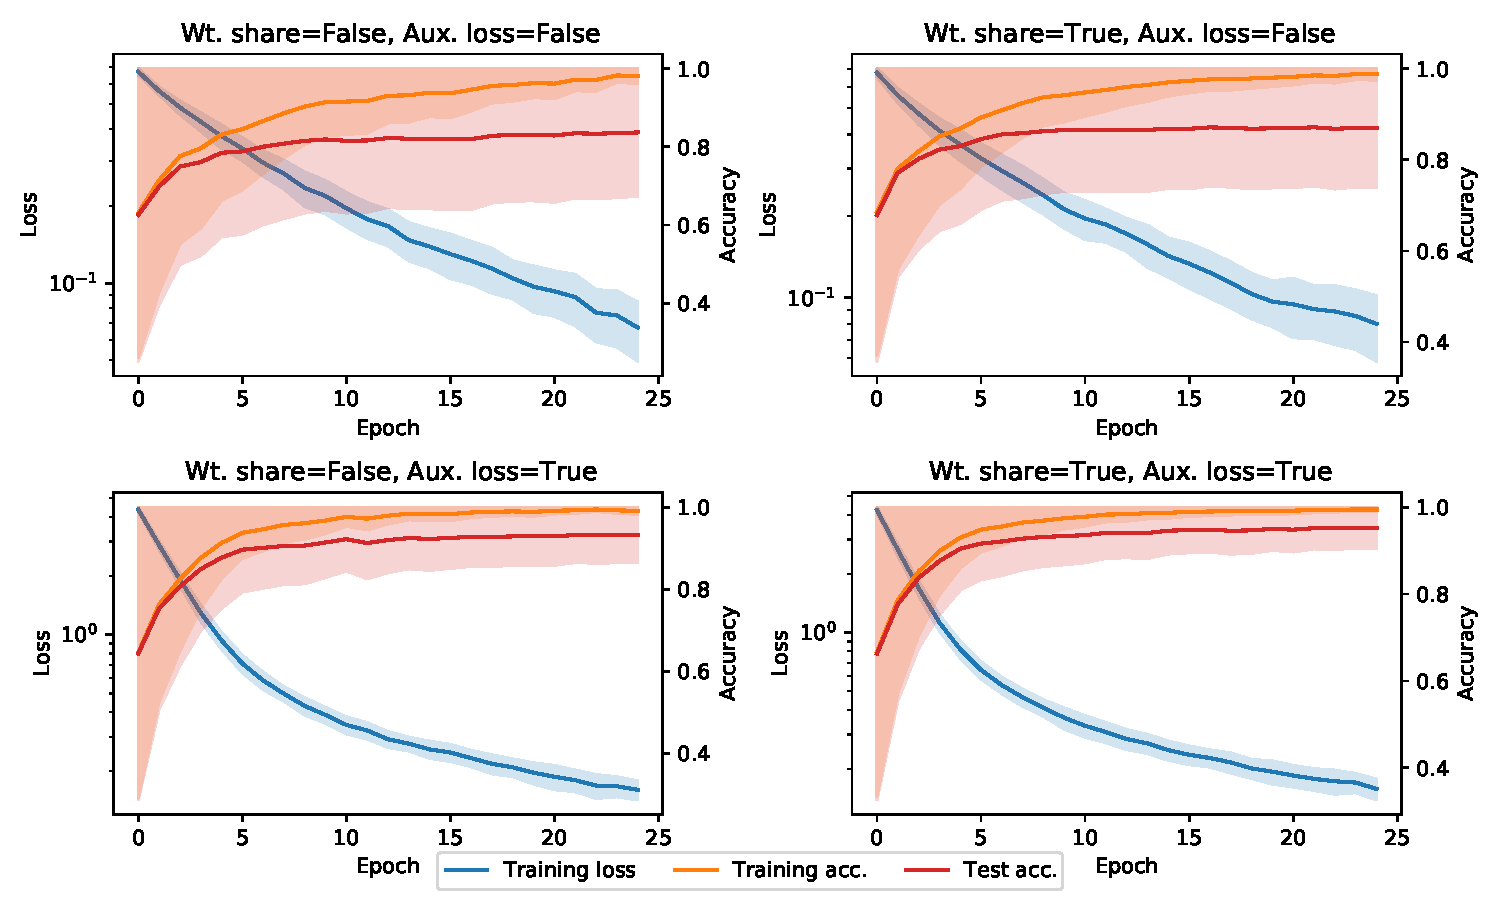
\includegraphics[width=\linewidth]{figures/avg_histories.pdf}
    \caption{Mean training curves for combinations of weight sharing and auxiliary loss with standard deviation fill ($N=32$).}
    \label{fig:training-curves}
\end{figure}


\section{Results}


\end{document}